

\section{Paper Summary}
This section gives a summary of the method presented in the paper, outlined in Figure \ref{fig:pipeline},
with an emphasis on explaining concepts that did not receive a lot of attention in the paper.

\begin{figure*}
    \centering
    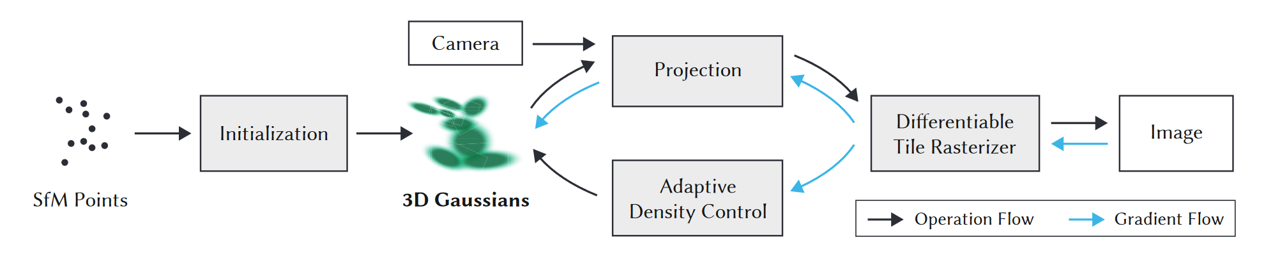
\includegraphics[width=\textwidth]{images/pipeline.png}
    \caption{The Gaussian splatting pipeline presented in the paper \cite[Fig. 2]{kerbl3DGaussianSplatting2023}.}
    \label{fig:pipeline}
\end{figure*}


\subsection{Representation}
The core idea of the paper is to represent the scene as a set of Gaussians.
Each Gaussian is defined by its position $\bm{\mu}$, its covariance matrix $\bm{\Sigma}$, its opacity $\alpha$ and its spherical harmonic coefficients $\bm{c}$ used to give it a view-dependent color, further discussed in Section \ref{sec:spherical_harmonics}.
The covariance is defined as
\begin{align}
    \bm{\Sigma} = \bm{R} \bm{S} \bm{S}^T \bm{R}^T,
\end{align}
where $\bm{R}$ is a rotation matrix stored as a quaternion $\bm{q}$ and $\bm{S}$ is a diagonal matrix containing the standard deviation of the Gaussian along each axis, stored as a vector $\bm{s}$.
To ensure that the covariance is positive definite, the values of $\bm{s}$ are passed through a sigmoid activation function, and quaternion $\bm{q}$ is normalized to ensure a proper rotation matrix.
In total, each Gaussian has 59 parameters, 3 for the position, 3 for the scale, 4 for the quaternion 1 for alpha and 48 for the spherical harmonic coefficients.

\subsection{Spherical Harmonics}
The first step in the rendering process, which is sort of overlooked in the paper, is to calculate the color of each Gaussian for a given view direction.
This is done using spherical harmonics, which can be seen as a spherical equivalent of the discrete cosine transform.
A key advantage of spherical harmonics is that they are differentiable and continuous.


\subsection{Projection}
\label{sec:projection}
The next step of the rendering pipeline, shown in Figure \ref{fig:pipeline}, is to project the Gaussians onto the image plane.
First, the Gaussians are transformed into the camera frame using a linear view transformation $\bm{W}$.
Then the Gaussians are projected onto the image plane using a pinhole projection.
This transformation is visualized by comparing Figure \ref{fig:proj_2a} and Figure \ref{fig:proj_2b}.


\begin{figure}[t]
    \centering
    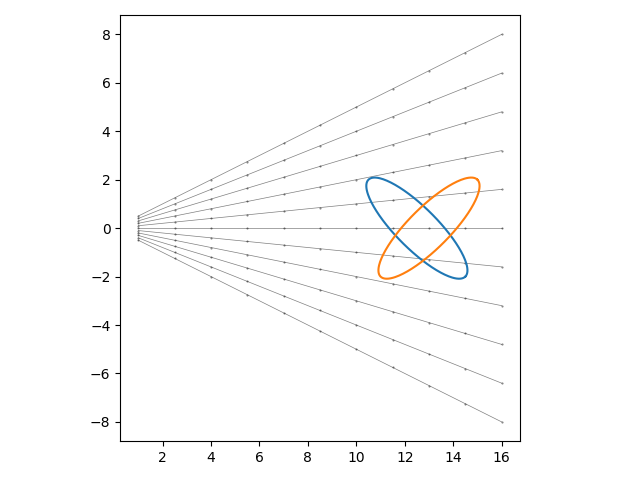
\includegraphics[width=\linewidth]{images/proja.png}
    \caption{Covariance ellipses of two Gaussians in the camera frame viewed from the side, with visualization of pixel rays.}
    \label{fig:proj_2a}
\end{figure}


Two key steps are performed to speed up the projection process.
First, instead of accurately projecting the Gaussians onto the image plane, a linear approximation is used where the center point is projected properly, but the covariance is updated given the following linear approximation,
\begin{align}
    \bm{\Sigma'} & = \bm{J} \bm{W} \bm{\Sigma} \bm{W}^T \bm{J}^T \label{eq:linear_approx}
\end{align}
where $\bm{J}$ is the Jacobian of the projection function.
The result of this approximation is visualized as the two dotted ellipses in Figure \ref{fig:proj_2b}.

A second significant speedup step is to flatten the projected Gaussians by only looking at their first two dimensions, resulting in 2D Gaussian with position $\bm{\mu}''$ and covariance $\bm{\Sigma}''$, visualized as a line in Figure \ref{fig:proj_2b}.
The key benefit of this is that the depth ordering of the Gaussians is identical for each pixel, which would not be the case otherwise as seen in Figure \ref{fig:proj_2b}.
This does however introduce a significant problem, where small changes in view direction can decide which Gaussian is in front of another Gaussian, resulting in strong popping artifacts, which the paper acknowledges \cite[Sec 7.4]{kerbl3DGaussianSplatting2023}.

\begin{figure}[htb]
    \centering
    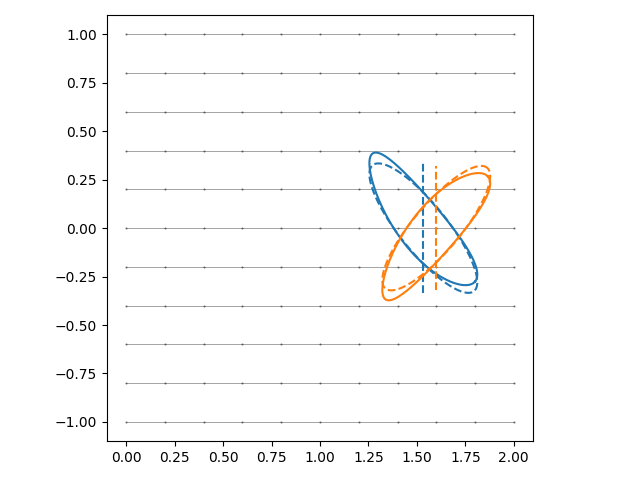
\includegraphics[width=\linewidth]{images/projb.png}
    \caption{The camera projection of Figure \ref{fig:proj_2a}. The dotted lines are the linear approximation of the Gaussians given Equation \ref{eq:linear_approx} and the vertical line is the simplification from removing the depth component}.
    \label{fig:proj_2b}
\end{figure}


\subsection{Rasterization Pipeline}
\label{sec:rasterization}
After the projection is complete, we have a set of 2D Gaussians that need to be rendered.
To achieve high frame rates, the paper uses a rasterization pipeline where the output image first is divided into 265 blocks.
Then they check which blocks each projected Gaussian overlaps with by drawing a circle with a radius of three times the largest eigenvalue of the covariance matrix, as illustrated in Figure \ref{fig:rendering}.
Gaussians outside the image plane or with a size smaller than one pixel are discarded, e.g. Gaussian D and E in Figure \ref{fig:rendering}
Then, they duplicate each Gaussian for each block it overlaps with and sort the Gaussians, first, according to the block they belong to and then according to their depth value.
This sorting is performed only once per iteration and they combine the block-index bits and depth bits into a single integer to perform both sorts in a single pass using parallel radix sort.

Each block is then responsible for non-overlapping sequential sections of the sorted output.
The color of each rendered pixel is calculated by iterating over the Gaussians in the block and blending them together using the alpha blending function given by
\begin{align}
    C   & = \sum_{i \in N} c_i a_i \prod_{j=1}^{i-1} (1-a_j)                                                     \\
    a_i & = \alpha_i \cdot exp(-\frac{1}{2}(\bm{x}-\bm{\mu}''_i)^T \bm{\Sigma}{''}_i^{-1} (\bm{x}-\bm{\mu}''_i))
    \label{eq:alpha_blending}
\end{align}
where $C$ is the resulting color, $c_i$ is the color of the $i$'th Gaussian calculated from the view direction and its spherical harmonic coefficients and $a_i$ is the evaluated opacity.

\begin{figure}
    \centering
    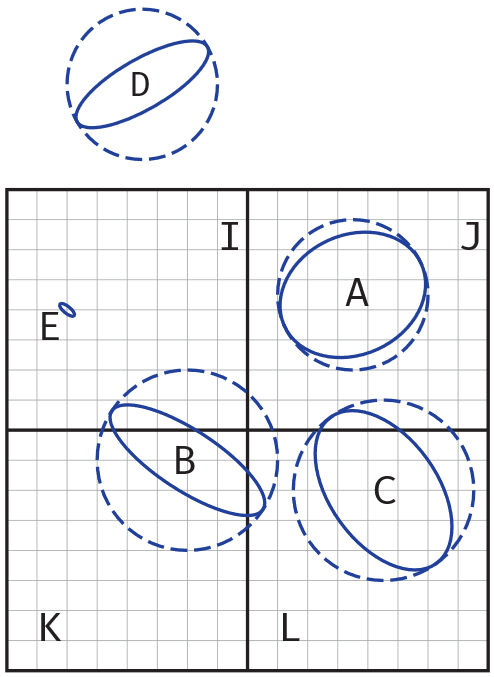
\includegraphics[width=0.6\linewidth]{images/rendering.png}
    \caption{Visualization of how Gaussian splats are rendered using multiple independent blocks. The dotted lines are from drawing a circle with a radius of three times the largest eigenvalue of the covariance matrix.}
    \label{fig:rendering}
\end{figure}


\subsection{Backpropagation}
The paper L1 loss together with structural dissimilarity index (D-SSIM) loss.
\begin{align}
    \mathcal{L} = (1 - \lambda) \mathcal{L}_1 + \lambda \mathcal{L}_{D-SSIM}
\end{align}
They have implemented custom CUDA accelerated backward pass functions for both the rasterization, projection and spherical harmonics steps that utilize cached information from the forward pass for speedup.



\subsection{Densification and Pruning}
In the paper, they use adaptive density control to generate Gaussians in areas where they are needed and remove unnecessary Gaussians to reduce memory usage.

For both the densification methods they simply check if a Gaussian has had large gradients with respect to position, i.e. if they have moved a lot around over the past 300 iterations.
They argue this happens when the Gaussian is moving to an area that is underrepresented or if the Gaussian is to big to fit the area it is in \cite[Sec 5.2]{kerbl3DGaussianSplatting2023}.
If the Gaussian is smaller than a certain threshold, it is cloned, and if it is larger than a certain threshold, it is split into two smaller Gaussians, as shown in Figure \ref{fig:densification}.

\begin{figure}
    \centering
    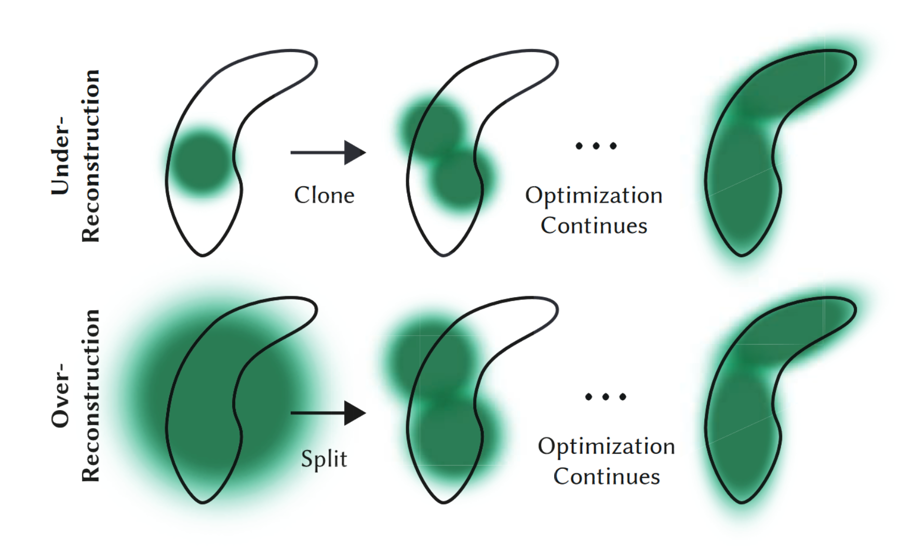
\includegraphics[width=\linewidth]{images/densification.png}
    \caption{The adaptive Gaussian densification scheme presented in the paper \cite[Fig. 4]{kerbl3DGaussianSplatting2023}.}
    \label{fig:densification}
\end{figure}
